\documentclass[tikz,crop]{standalone}

\usepackage[T1]{fontenc}
\usepackage[tt=false,type1=true]{libertine}
\usepackage[varqu]{zi4}
\usepackage{newtxmath}
\usepackage[dvipsnames]{xcolor}
\usepackage{tikz,listings}
\usepackage{bbding}
\usetikzlibrary{arrows,fit,positioning,shadows,shapes,shapes.arrows}

\lstset{
    % backgroundcolor=\color{backcolour},
    % stringstyle=\color{codepurple},
    % commentstyle=\color{codegreen},
    keywordstyle=\bfseries\color{magenta},
    numberstyle=\tiny\color{codegray},
    basicstyle=\ttfamily\tiny,
    % captionpos=b,
    escapeinside={/@}{@/},
    % breakatwhitespace=false,
    % breaklines=true,
    % keepspaces=true,
    % numbers=left,
    % numbersep=5pt,
    % showspaces=false,
    % showstringspaces=false,
    % showtabs=false,
    % tabsize=2
}
\colorlet{ml-model-bg}{CornflowerBlue!10}
\colorlet{maru}{Green}
\colorlet{batsu}{OrangeRed!80}
\colorlet{tadashi}{Red}
\def\maru{{\color{maru}\CheckmarkBold}}
\def\batsu{{\color{batsu}\XSolidBold}}
\newbox\trainpy
\newbox\inputc
\newbox\outputc

\begin{document}


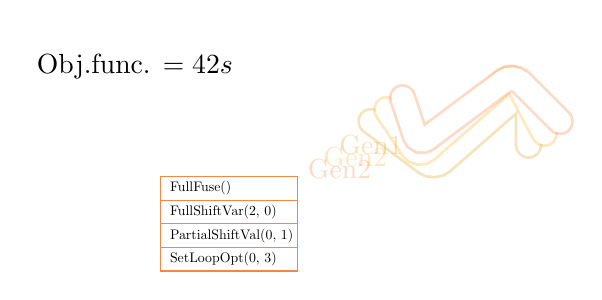
\begin{tikzpicture}

  %%% Begin Transformations %%%
  % XOXO
  \begin{scope}[xscale=2, yscale=1.5,
    foo/.style={
      line width=10pt,
      opacity=0.3,
      line cap=round,
      rounded corners,
    },
    bar/.style={
      line width=8pt,
      opacity=1,
      line cap=round,
      draw=white,
      rounded corners,
    }]
    \def\wiggly#1#2#3#4{
      \draw[foo, #4] (#1, #2)
      \foreach \x/\y in #3{ -- (\x, \y)} ;
      \draw[bar] (#1, #2)
      \foreach \x/\y in #3{ -- (\x, \y)} ;
    }
    \wiggly{0.0}{0.2}{{0.4/-0.2,  1.0/0.5, 1.0/0.0}}{Goldenrod}
    \wiggly{0.1}{0.3}{{0.3/-0.1,  0.9/0.6, 1.1/0.1}}{Dandelion}
    \wiggly{0.2}{0.4}{{0.3/-0.0,  0.9/0.6, 1.2/0.2}}{Peach}
    \node[foo,Goldenrod] at (0.0, 0.0) {Gen1};
    \node[foo,Dandelion] at (-0.1, -0.1) {Gen2};
    \node[foo,Peach] at (-0.2, -0.2) {Gen2};

    % \draw[foo, Dandelion] (-0.5,-0.4) .. controls (-0.7,-0.8) .. (-0.8,0.0);
    % \draw[bar]            (-0.5,-0.4) .. controls (-0.7,-0.8) .. (-0.8,0.0);
    % \node[Dandelion] at (-0.7, -0.8) {Gen2};

    % \draw[foo, Peach] (0.7,-0.0) .. controls (1.0,-0.7) .. (0.6,-0.4);
    % \draw[bar]        (0.7,-0.0) .. controls (1.0,-0.7) .. (0.6,-0.4);
    % \node[Peach] at (1.0, -0.7) {Gen3};
    \foreach [
      evaluate=\i as \xmaru using rand,
      evaluate=\i as \xbatsu using rand,
      evaluate=\i as \ymaru using rand,
      evaluate=\i as \ybatsu using rand,
      evaluate=\xmaru \ymaru as \smaru using (1.5-sqrt(\xmaru*\xmaru+\ymaru*\ymaru)),
      evaluate=\xbatsu \ybatsu as \sbatsu using (1.5-sqrt(\xbatsu*\xbatsu+\ybatsu*\ybatsu)),
      remember=\xmaru as \lxmaru (initially 0),
      remember=\ymaru as \lymaru (initially 0),
      ] \i in {1,2,...,40}{
      \node[scale=\sbatsu, opacity=1.2-\sbatsu] at (\xbatsu, \ybatsu) (batsu-\i) {\batsu};
      \node[scale=\smaru, opacity=1.2-\smaru] at (\xmaru, \ymaru) (maru-\i) {\maru};
    }
  \end{scope}
  %%% End Transformations %%%
  %%% Begin Samples %%%
  \path node [
    scale=0.5,
    draw=Peach,
    fill=white,
    rectangle split,
    rectangle split parts=4,
    rectangle split part align=left,
  ] at (-1.8cm, -1cm)
    (legend) {         \textcolor{SpringGreen}{\CheckmarkBold}  FullFuse()
    \nodepart{two}     \textcolor{SpringGreen}{\CheckmarkBold}  FullShiftVar(2, 0)
    \nodepart{three}   \textcolor{Red}{\XSolidBold}  PartialShiftVal(0, 1)
    \nodepart{four}    \textcolor{SpringGreen}{\CheckmarkBold}  SetLoopOpt(0, 3)
  }
  ;
  %%% End Samples %%%
  %%% BEGIN Reward %%%
  \node at (-3,1) {Obj.func. $=42s$};
  %%% END Reward %%%

\end{tikzpicture}
\end{document}
